
% The \section{} command formats and sets the title of this
% section. We'll deal with labels later.
\section{Introduction}
\label{sec:intro}

Linear, polynomial, and other forms of regression analysis are commonly
used in the field of statistics in order to fit a function to a data set. Produced
functions can be used to predict behavior at arbitrary input values. Typically,
regression analysis is used upon data sets for which the approximate
function \textit{type} (e.g. linear, quadratic, etc.) is known. Traditional
regression analysis is not well-suited, however, for data sets which
approximate an unknown function type.

One tried solution for such scenarios is symbolic regression by way of
a genetic algorithm --- an algorithm that generates sets of candidate
solutions, randomly splices together traits from pairs of fit "parents"
into "children" over successive generations, and occasionally mutates
pieces of those candidates, until a strongly fit solution is found.

In our paper we introduce expression trees as a means of representing
functional expressions in such a way that they can be easily spliced by
a genetic algorithm. We discuss our own implementation of symbolic
regression for two known data sets representing unknown functions,
inspired by the work of John Koza \cite{koza}.

\begin{figure}[ht]
	\centering
	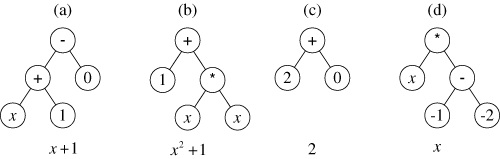
\includegraphics[width=0.47\textwidth]{figs/exprtrees.jpg}
	\caption{An example set of expression trees representing functions \cite{fig:gpquadraticexample}.}
	\label{fig:gpquadraticexample}
\end{figure}

